\documentclass[12pt, a4paper]{article}

\usepackage[hmargin=2.5cm, vmargin=2cm]{geometry}
\usepackage{amsthm, amssymb, mathtools, yhmath, graphicx}
\usepackage{fontspec, type1cm, titlesec, titling, fancyhdr, tabularx}
\usepackage{color}
\usepackage{unicode-math}
\usepackage{float}
\usepackage{hhline}
\usepackage{comment}
\usepackage[abbreviations]{siunitx}
\usepackage{csvsimple}
\usepackage{subcaption}
\usepackage{cleveref}
\usepackage{listings}
\definecolor{mygreen}{rgb}{0,0.6,0}
\lstset{
  basicstyle=\footnotesize\ttfamily,
  breaklines=true,
  keywordstyle=\color{blue},
  numbers=left,
  numberstyle=\tiny\color{mygray},
  commentstyle=\color{mygreen}, 
}

\usepackage[CheckSingle, CJKmath]{xeCJK}
\usepackage{CJKulem}
\usepackage{enumitem}
\usepackage{tikz}
\usepackage[siunitx]{circuitikz}
\usepackage{wrapfig}
\usepackage{sourcecodepro}
%\setCJKmainfont[BoldFont=cwTex Q Hei]{cwTex Q Ming}
%\setCJKsansfont[BoldFont=cwTex Q Hei]{cwTex Q Ming}
%\setCJKmonofont[BoldFont=cwTex Q Hei]{cwTex Q Ming}
\setCJKmainfont[BoldFont=cwTeX Q Hei]{cwTeX Q Ming}
\setmonofont{Source Code Pro}

\def\normalsize{\fontsize{12}{18}\selectfont}
\def\large{\fontsize{14}{21}\selectfont}
\def\Large{\fontsize{16}{24}\selectfont}
\def\LARGE{\fontsize{18}{27}\selectfont}
\def\huge{\fontsize{20}{30}\selectfont}

\newtheorem{lemma}{Lemma}

%\titleformat{\section}{\bf\Large}{\arabic{section}}{24pt}{}
%\titleformat{\subsection}{\large}{\arabic{subsection}.}{12pt}{}
%\titlespacing*{\subsection}{0pt}{0pt}{1.5ex}

\parindent=24pt

\DeclarePairedDelimiter{\abs}{\lvert}{\rvert}
\DeclarePairedDelimiter{\norm}{\lVert}{\rVert}
\DeclarePairedDelimiter{\inpd}{\langle}{\rangle}
\DeclarePairedDelimiter{\ceil}{\lceil}{\rceil}
\DeclarePairedDelimiter{\floor}{\lfloor}{\rfloor}

\newcommand{\unit}[1]{\:(\text{#1})}
\newcommand{\df}[1]{\mathop{}\!\mathrm{d^#1}}
\newcommand{\img}{\mathrm{i}}
\newcommand{\dD}{\mathrm{d}}
\newcommand{\dI}{\,\mathrm{d}}

\title{ \bf {\Huge Signal and System}\\ MATLAB Homework \#1}
\author{B02901178 江誠敏}

\begin{document}

\maketitle

\begin{enumerate}
  \item Use the command stem to plot $x_1[n]$ and $x_2[n]$. \\[12pt]
    Here is the code I used.
    \lstinputlisting[language=Octave, lastline=19]{p1.m}
    And here is the plots.

    \begin{figure}[H]
      \begin{subfigure}{0.45\textwidth}
        \centering
        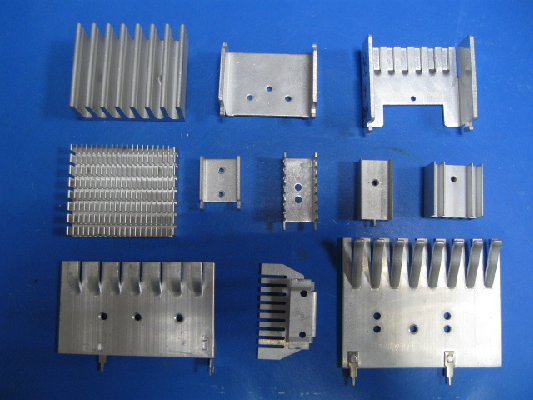
\includegraphics[width=\textwidth]{p1.jpg}
        \caption{Plot of $x_1[n]$}
      \end{subfigure}
      \begin{subfigure}{0.45\textwidth}
        \centering
        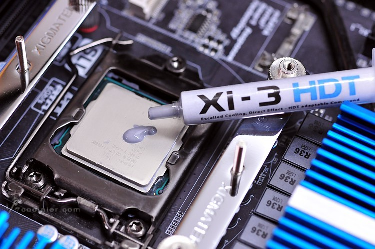
\includegraphics[width=\textwidth]{p2.jpg}
        \caption{Plot of $x_2[n]$}
      \end{subfigure}
    \end{figure}
  \item Use the command conv to compute (1). \\[12pt]
    Continue from (1)
    \lstinputlisting[language=Octave, firstline=21]{p1.m}
    And here is the plot.
    \begin{center}
    \begin{figure}[H]
      \centering
      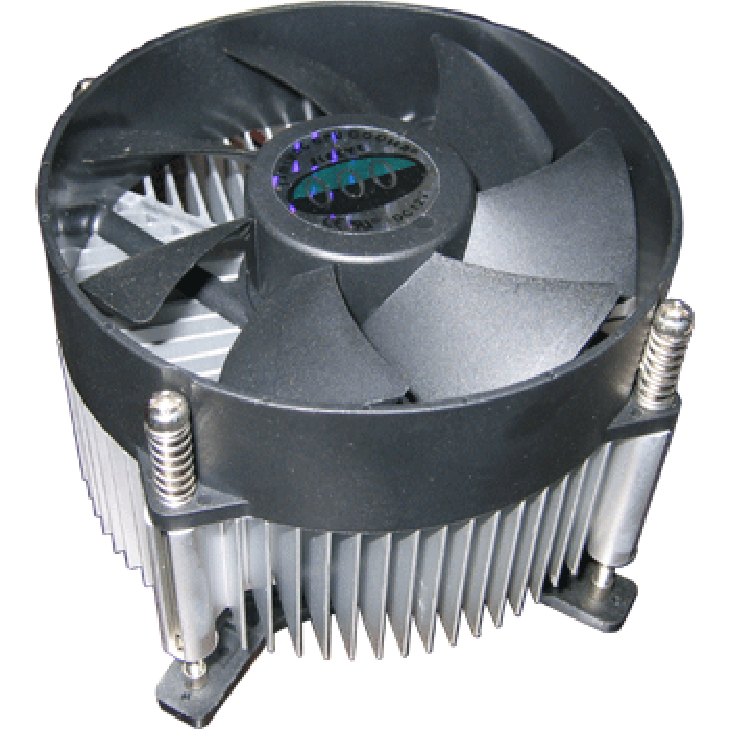
\includegraphics[width=0.6\textwidth]{p3.jpg}
      \caption{Plot of $y = x1 * x2$}
    \end{figure}
    \end{center}

  \item Write a MATLAB function my1conv.m to compute (1) directly and plot y when
    \[ x_1 = x_2 = \begin{cases}
        1, & n = 1, 2, \cdots, 500 \\
        0, & \text{elsewhere}
    \end{cases} \]
    \\[12pt]
    The function is at the file \texttt{my1conv.m}, and then use the code below
    \lstinputlisting[language=Octave]{p3.m}
    to compute the result. Below is the plot.
    \begin{center}
    \begin{figure}[H]
      \centering
      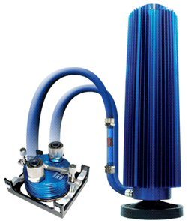
\includegraphics[width=0.6\textwidth]{p4.jpg}
      \caption{Plot of $y = x1 * x2$}
    \end{figure}
    \end{center}

  \item Write a MATLAB function my2conv.m to compute (1) using (2) and plot y when
    \[ x_1 = \begin{cases}
        1, & n = 1, 2, \cdots, 500 \\
        0, & \text{elsewhere}
    \end{cases} \] and
    \[ x_2 = \begin{cases}
        1, & n = 1, 2, \cdots, 1001 \\
        0, & \text{elsewhere}
    \end{cases} \]
    \\[12pt]
    The function is at the file \texttt{my2conv.m}, and then use the code below
    \lstinputlisting[language=Octave]{p4.m}
    to compute the result. Below is the plot.
    \begin{center}
    \begin{figure}[H]
      \centering
      \includegraphics[width=0.6\textwidth]{p5.jpg}
      \caption{Plot of $y = x1 * x2$}
    \end{figure}
  \end{center}
\end{enumerate}
\end{document}

